\documentclass{article}
\usepackage{tikz}
\usetikzlibrary{automata,positioning}

\begin{document}

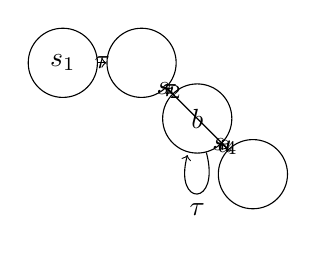
\begin{tikzpicture}[node distance=1cm]
    \node[state] (s1) {$s_1$};
    \node[state] (s2) [right of=s1] {};
    \node[state] (s3) [below right of=s2] {};
    \node[state] (s4) [below right of=s3] {};
    
    \path[->]
        (s1) edge node {$\tau$} (s2)
        (s2) edge node {$s_2$} (s3)
        (s3) edge node {$a$} (s4)
        (s4) edge node {$b$} (s2)
        (s2) edge node {$\tau$} (s3)
        (s3) edge [loop below] node {$\tau$} ()
        (s4) edge node {$s_4$} (s3);
\end{tikzpicture}

\end{document}